\documentclass[border=10pt]{standalone}
\usepackage{tikz}
\usetikzlibrary{shapes.geometric}

\tikzset{
  parallelogram/.style={
    draw,
    fill=black!20,
    minimum width=3cm,
    minimum height=2cm,
    inner sep=0pt,
    outer sep=0pt,
    shape border rotate=#1
  }
}

\begin{document}

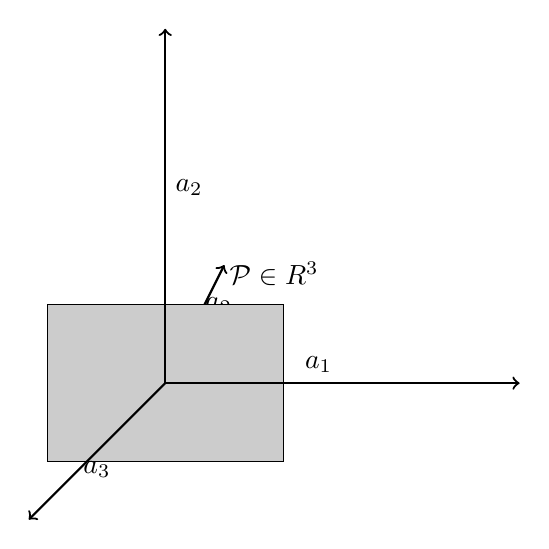
\begin{tikzpicture}[scale=1.5]

% Define coordinates for the parallelogram in R^2
\coordinate (O) at (0,0);
\coordinate (a1) at (1,0);
\coordinate (a2) at (0.5,1);

% Draw the parallelogram
\node[parallelogram=0] at (O) {};
\draw[->,thick] (O) -- node[above left] {$a_1$} (a1);
\draw[->,thick] (O) -- node[above right] {$a_2$} (a2);
\node at (0.5,-0.5) {$\mathcal{P}\in\mathbb{R}^2$};

% Define coordinates for the parallelepiped in R^3
\coordinate (O) at (0,0,0);
\coordinate (a1) at (3,0,0);
\coordinate (a2) at (0,3,0);
\coordinate (a3) at (0,0,3);

% Draw the parallelepiped
\node[parallelogram=45] at (O) {};
\draw[->,thick] (O) -- node[above left] {$a_1$} (a1);
\draw[->,thick] (O) -- node[above right] {$a_2$} (a2);
\draw[->,thick] (O) -- node[below] {$a_3$} (a3);
\node at (1.5,1.5,1.5) {$\mathcal{P}\in\mathbb{R}^3$};

\end{tikzpicture}

\end{document}